\ifpdf
\graphicspath{ {Chapters/COMPASS/Figs/} }
\section{COMPASS}

\begin{frame}
  %\frametitle{}

  \begin{figure}
    \centering
    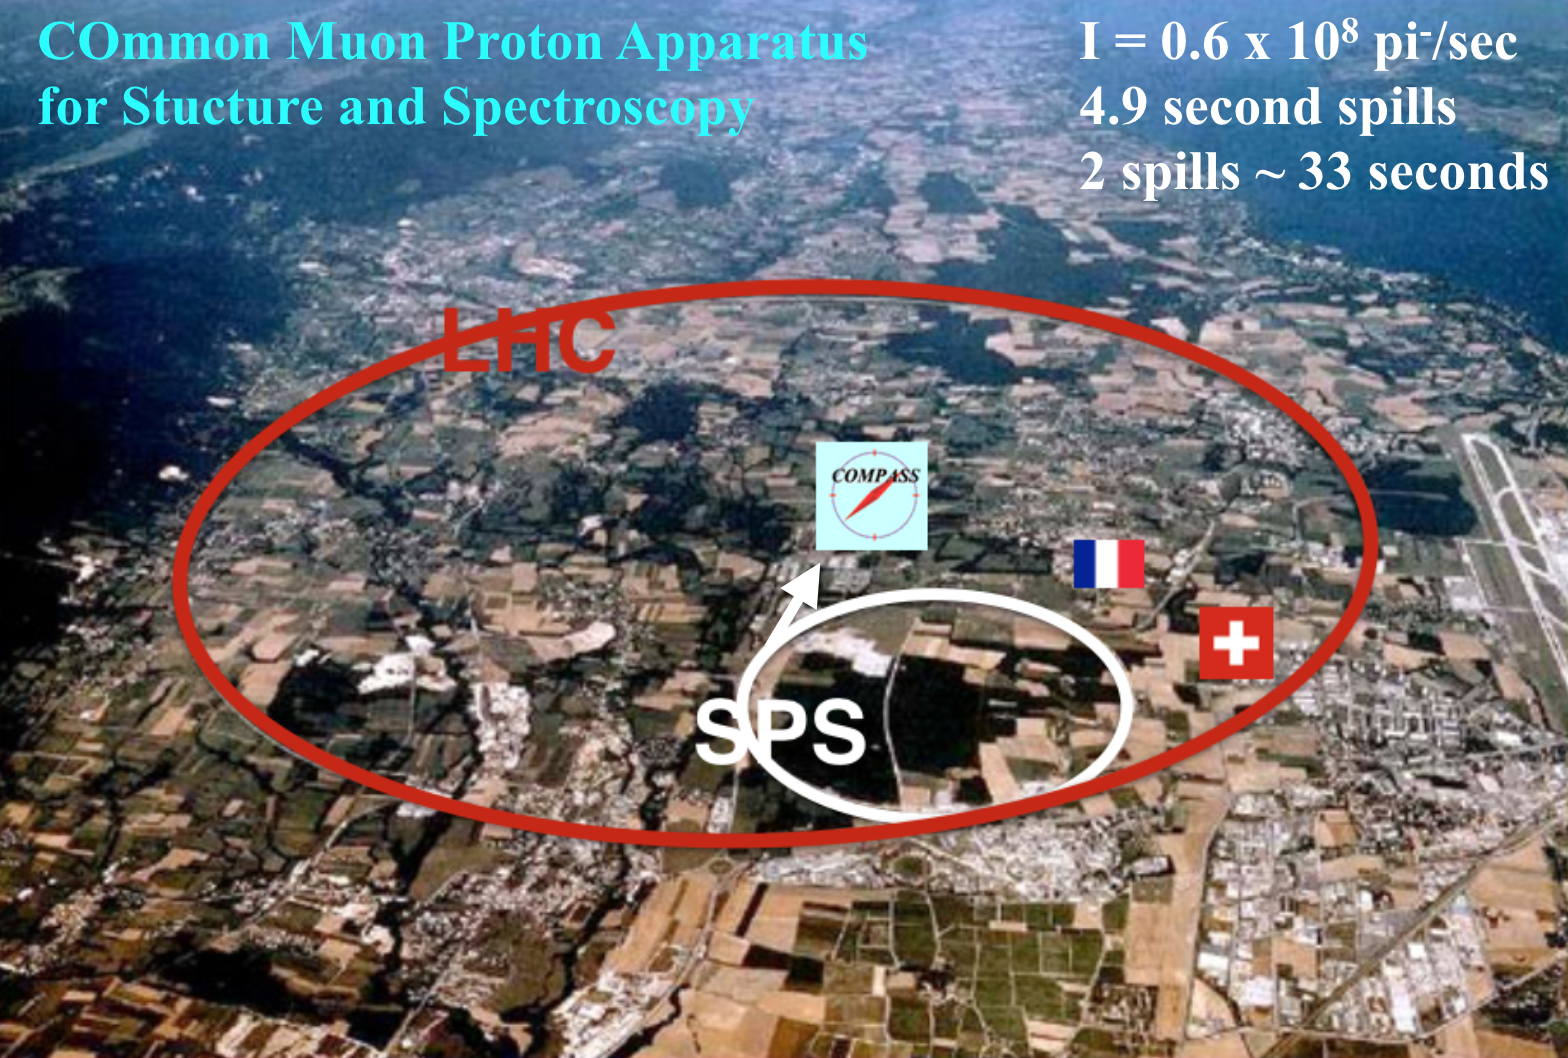
\includegraphics[width=\textwidth]{COMPASS_birdsEye}
  \end{figure}
\end{frame}


%\subsection{Spectrometer}
\begin{frame}
  \frametitle{COMPASS Spectometer}
  
  \begin{figure}
    \centering
    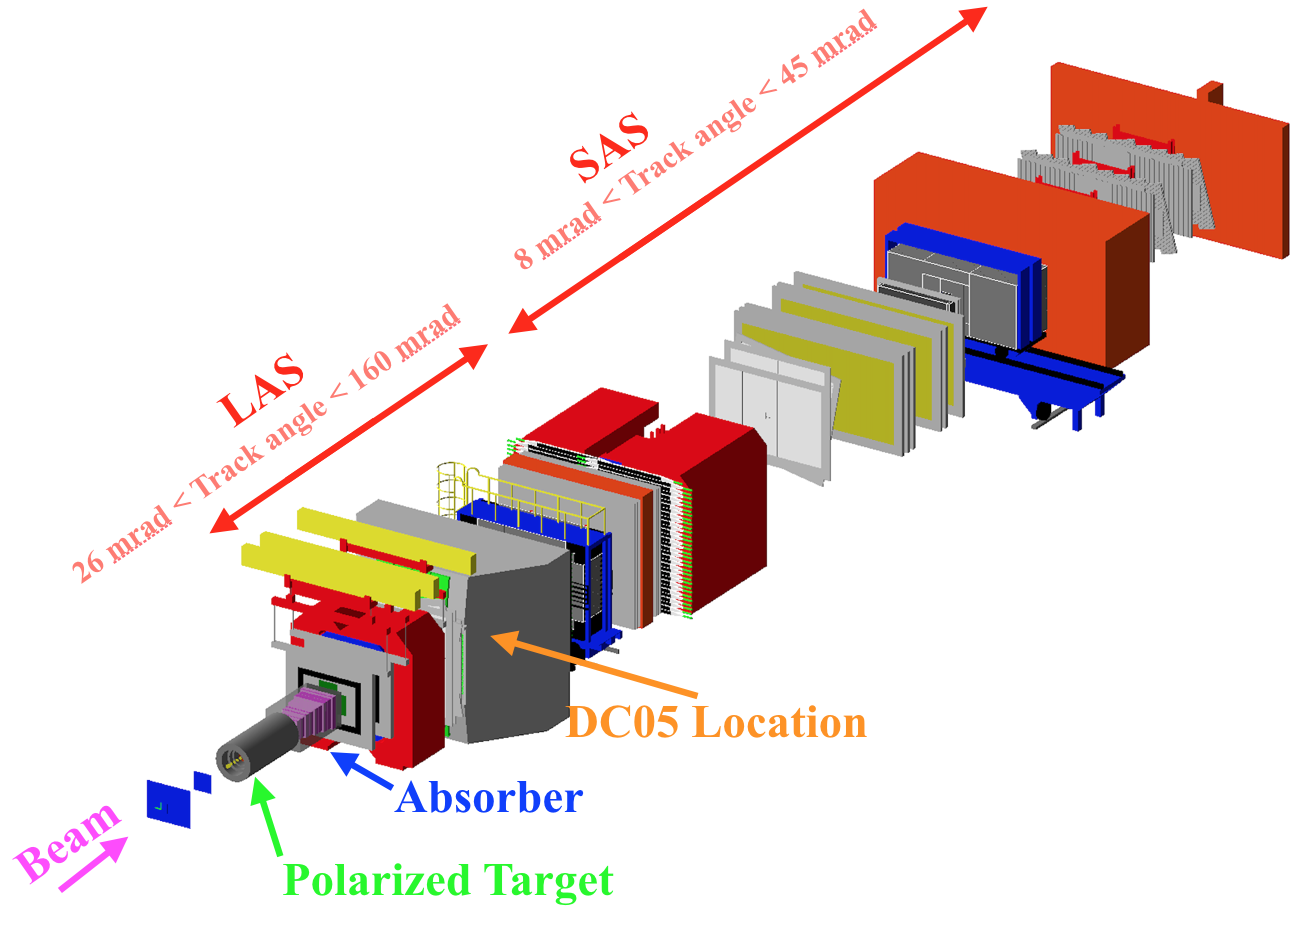
\includegraphics[width=0.79\textwidth]{COMPASS_spec}
  \end{figure}

  \begin{itemize}
  \item $\sim$ 60m long
  \item Largest above ground detector in the world
  \end{itemize}
\end{frame}


%\subsection{2015 Drell-Yan Measurement}
\begin{frame}
  \frametitle{2015 COMPASS Data Taking}

  \begin{itemize}
  \item 190 GeV/c $\pi^-$ beam
  \item Transversely polarized NH$_3$ (proton) target
    \begin{itemize}
    \item Kept in frozen spin mode at 70mK
    \item Polarization $\sim$ 73$\%$
    \item Target cell polarization flipped each week
    \end{itemize}
  \item Hadron absorber downstream of target
    \begin{itemize}
    \item Al and W beam plugs
    \item $\sim$ 7.5 interaction lengths
    \end{itemize}
  \end{itemize}

  \begin{figure}
    \centering
    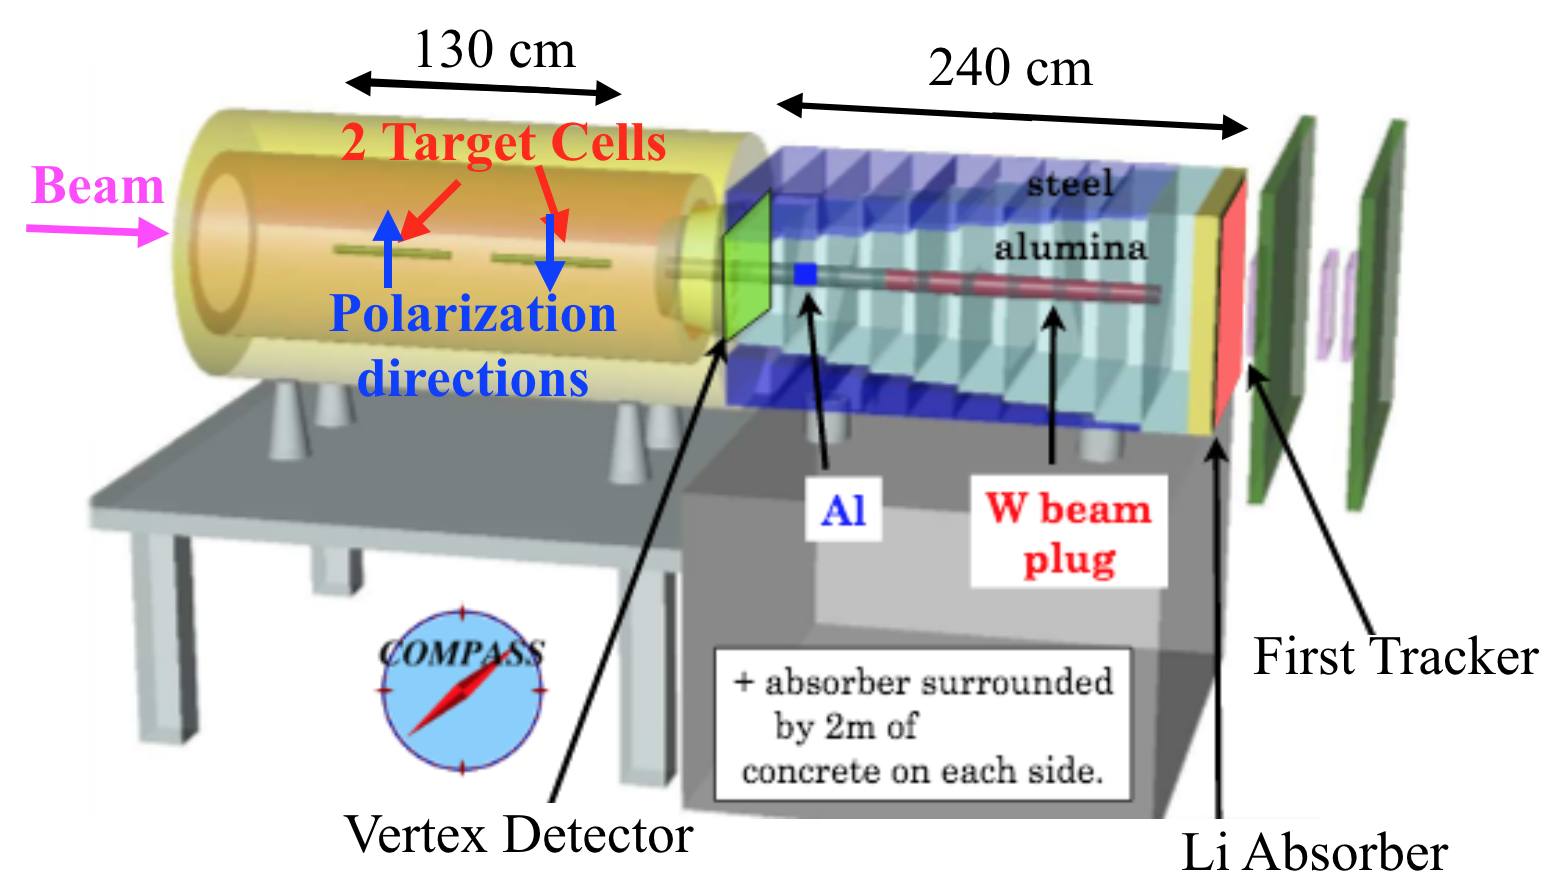
\includegraphics[width=0.65\textwidth]{Target_Absorb}
  \end{figure}
\end{frame}
